\documentclass{standalone}
\usepackage{tikz}
\begin{document}
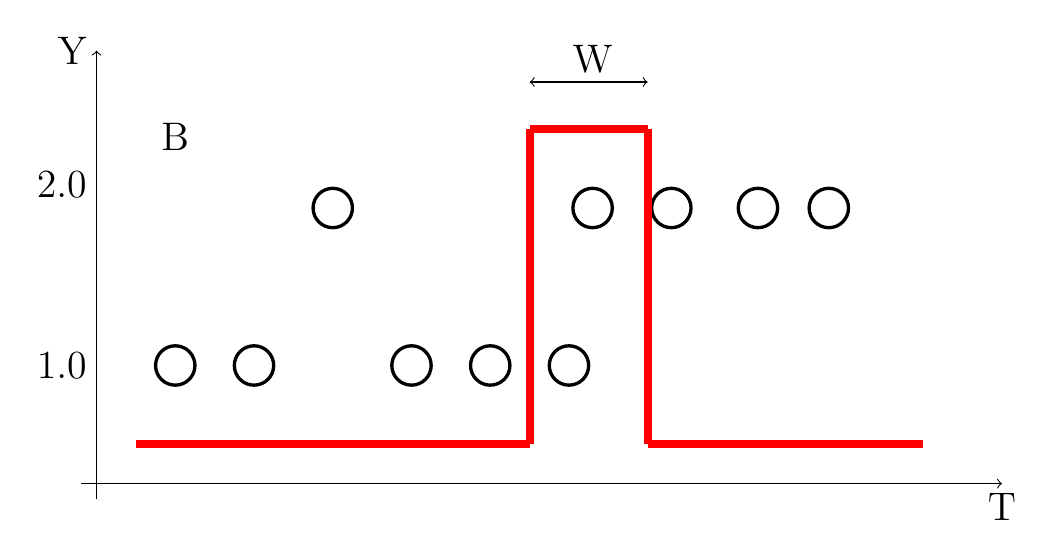
\begin{tikzpicture}[scale=1.0, xscale=1]
\def\rad{0.25}
\def\step{3}
%    \draw [<->] (0, 5) node [left] {$y$} -- (0,0) -- (15, 0) node [below right] at (15.5,-0.3) {$t$};
%\draw [->] (0,-0.5) -- (9,-0.5);
\draw [->] (-1-2, -0.7) -- (-1-2,5) node[left] {\Large Y};
\draw [->] (-1.2-2, -0.5) -- (8.5, -0.5) node[below] {\Large T};

\node[left] at (-3, 1) {\Large 1.0};
\node[left] at (-3, 3.3) {\Large 2.0};

\draw[fill=white, very thick] (-2, 1) circle (\rad);
\draw[fill=white, very thick] (-1, 1) circle (\rad);
\draw[fill=white, very thick] (0, \step) circle (\rad);
\draw[fill=white, very thick] (1, 1) circle (\rad);
\draw[fill=white, very thick] (2, 1) circle (\rad);
\draw[fill=white, very thick] (3, 1) circle (\rad);
\draw[fill=white, very thick] (3.3, \step) circle (\rad);
\draw[fill=white, very thick] (4.3, \step) circle (\rad);
\draw[fill=white, very thick] (5.4, \step) circle (\rad);
\draw[fill=white, very thick] (6.3, \step) circle (\rad);
%\draw[fill=white, very thick] (7.3, \step) circle (\rad);

%\draw[black, dashed] (4.5,0) -- (4.5, 4.5);

\draw[red, line width = 1mm] (-0.5-2, 0) -- (2.5, 0);
\draw[red, line width = 1mm] (2.5, 0) -- (2.5, 4);
\draw[red, line width = 1mm] (2.5, 4) -- (4.0, 4);
\draw[red, line width = 1mm] (4.0, 4) -- (4.0, 0);
\draw[red, line width = 1mm] (4.0, 0) -- (7.5,0);

\draw[<->] (2.5, 4.6) -- (4.0, 4.6);
\node[above] at (3.3, 4.6) {\Large W};

\node[above] at (-2, 3.6) {\Large B};

\end{tikzpicture}
\end{document}
